\chapter{Project Initiation}

\section{Introduction}

This project develops a comprehensive PlantUML-based diagramming platform combining individual productivity tools with community collaboration features. The web-based solution enables creating, editing, and sharing PlantUML diagrams while fostering collaborative learning environments.

The platform targets developers, software architects, system designers, and educational institutions requiring efficient technical diagram creation and visual documentation tools.

The project follows agile development using Scrum framework for iterative development and continuous feedback integration.

\section{Requirements Analysis}

\subsection{System Actors}

\textbf{Primary Actors:}
\begin{itemize}
    \item \textbf{User}: Authenticated individuals with full platform access including workspace management and community interaction
\end{itemize}

\textbf{Secondary Actors:}
\begin{itemize}
    \item \textbf{AI System}: Intelligent assistant providing code editing assistance
    \item \textbf{PlantUML Server}: External service for diagram rendering
\end{itemize}

\subsection{Core Requirements}

\subsubsection{Functional Requirements}
\begin{itemize}
    \item \textbf{Authentication}: OAuth via Google/GitHub with cross-device persistence
    \item \textbf{Project Management}: Complete CRUD operations, sharing, and bulk export
    \item \textbf{Workspace}: Interactive editor with real-time rendering and AI assistance
    \item \textbf{Community}: Project exploration, commenting, liking, and forking
    \item \textbf{Profile}: User management and public portfolio display
\end{itemize}

\subsubsection{Non-Functional Requirements}
\begin{itemize}
    \item \textbf{Performance}: Page loads <3s, diagram rendering <5s, real-time syntax highlighting and rendering
    \item \textbf{Security}: HTTPS/TLS encryption, OAuth 2.0 authentication, input validation, XSS/CSRF protection, secure code execution sandboxing
    \item \textbf{Usability}: Responsive design across devices, WCAG 2.1 Level AA accessibility compliance, intuitive visual interface design
    \item \textbf{Editor Experience}: Syntax highlighting, intelligent autocomplete with context awareness, real-time error detection
    \item \textbf{SEO \& Discoverability}: Server-side rendering (SSR) for search engine optimization, semantic HTML structure
\end{itemize}

\section{Project Management}

\subsection{Scrum Rol}

\begin{table}[H]
    \centering
    \begin{tabular}{|l|l|}
        \hline
        \textbf{Role}          & \textbf{Member(s)}             \\ \hline
        Product Owner          & Issam Mekni                   \\ \hline
        Scrum Master           & Issam Mekni                   \\ \hline
        Development Team       & Issam Mekni, Souhaieb Askri   \\ \hline
    \end{tabular}
    \caption{Scrum team roles}
\end{table}
\subsection{Product Backlog}

The product backlog represents a prioritized list of features and requirements derived from stakeholder needs and market analysis. Each backlog item follows the user story format and includes priority classification using MoSCoW method (Must have, Should have, Could have, Won't have this time).

\begin{longtable}{|p{0.7cm}|p{3.6cm}|p{0.7cm}|p{9cm}|p{1.5cm}|}
    \caption{Product Backlog with User Stories } \label{tab:product_backlog} \\
    \hline
    \textbf{ID} & \textbf{Feature} & \textbf{Sub-ID} & \textbf{User Story} & \textbf{Priority} \\
    \hline
    \endfirsthead
    
    \multicolumn{5}{c}%
    {{\bfseries \tablename\ \thetable{} -- continued from previous page}} \\
    \hline
    \textbf{ID} & \textbf{Feature} & \textbf{Sub-ID} & \textbf{User Story} & \textbf{Priority} \\
    \hline
    \endhead
    
    \hline \multicolumn{5}{|r|}{{Continued on next page}} \\ \hline
    \endfoot
    
    \hline
    \endlastfoot
    
    \csvreader[no head, late after line=\\]{./backlog1.csv}{}%
    {\csvcoli & \csvcolii & \csvcoliii & \csvcoliv & \csvcolv}
    \end{longtable}
\subsection{Global Use Case Diagram}

\begin{figure}[H]
    \centering
    \includegraphics[width=0.85\textwidth]{./conception/global_use_case_diagram.png}
    \caption{Global Use Case Diagram}
    \label{fig:global_use_case}
\end{figure}

\subsection{Sprint Planning}

The project is organized into six strategic sprints, each focusing on specific functional areas and building upon previous deliverables. The total project duration is designed to fit within 3.5 months (14 weeks) with efficient resource allocation and parallel development activities.

\begin{table}[h!]
    \centering
    \begin{tabular}{|c|l|l|c|}
        \hline
        \textbf{Sprint} & \textbf{Focus Area}                                & \textbf{Backlog Features}                                   & \textbf{Weeks} \\ \hline
        I              & Infrastructure Setup                               & N/A                                                     & 2                                   \\ \hline
        II             & Authentication and Landing Page                    & 1,2                              & 3                                 \\ \hline
        III            & Project Management                                 & 3                            & 3                                   \\ \hline
        IV             & Diagram and Project Management                     & 4,5                            & 3                                   \\ \hline
        V              & Community Interaction and Profiles                 & 6 ,7                          & 3                                   \\ \hline
    \end{tabular}
    \caption{Scrum Sprint Planning with Estimated Durations}
\end{table}

\subsection{Class Diagram}

The database implements a normalized schema supporting core application functionality:

\begin{figure}[H]
  \centering
  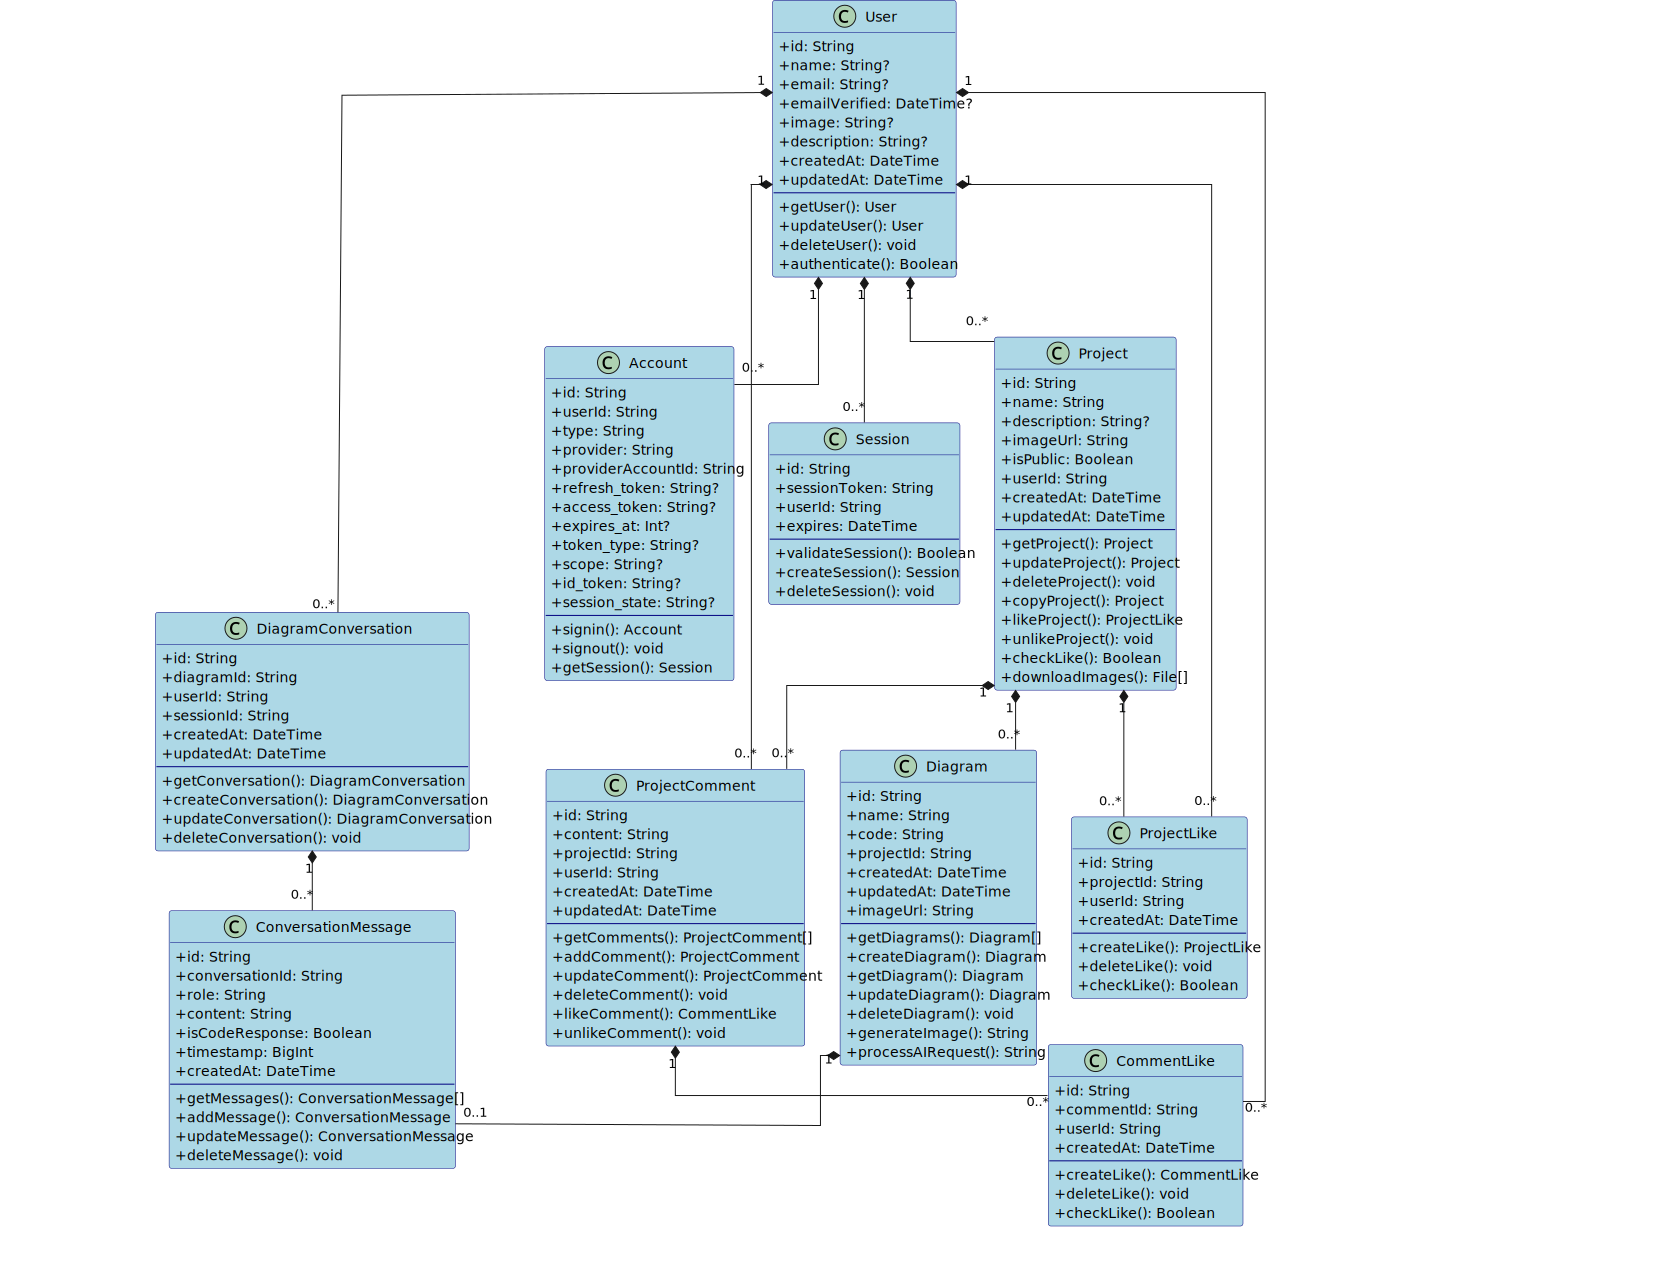
\includegraphics[width=0.85\textwidth]{conception/SprintI/class_diagram2.png}
  \caption{Class Diagram}
  \label{fig:class_diagram}
\end{figure}
\section{System Architecture}

\subsection{Deployment Overview}

\begin{figure}[H]
    \centering
    \includegraphics[width=0.85\textwidth]{./conception/deployement_diagram.png}
    \caption{Deployment Architecture}
    \label{fig:deployment}
\end{figure}

\subsection{Technology Stack}

\begin{table}[H]
    \centering
    \begin{tabular}{|p{3cm}|p{8cm}|}
        \hline
        \textbf{Category} & \textbf{Technologies} \\ \hline
        
         Frontend & 
        \includegraphics[width=0.6cm]{pictures/web/logo/next-js.png} Next.js, 
        \includegraphics[width=0.6cm]{pictures/web/logo/reactts-svgrepo-com.png} React, 
        \includegraphics[width=0.6cm]{pictures/web/logo/typescript-official-svgrepo-com.png} TypeScript, \newline
        \includegraphics[width=0.6cm]{pictures/web/logo/tailwind-svgrepo-com.png} Tailwind CSS \\ \hline
        
         Backend & 
        \includegraphics[width=0.6cm]{pictures/web/logo/node-svgrepo-com.png} Node.js, 
        \includegraphics[width=0.6cm]{pictures/web/logo/next-authe.png} NextAuth.js, \newline
        \includegraphics[width=0.6cm]{pictures/web/logo/prisma.png} Prisma ORM \\ \hline
        
         Database & 
        \includegraphics[width=0.6cm]{pictures/web/logo/pgsql-svgrepo-com.png} PostgreSQL \\ \hline
        
         AI Integration & 
        \includegraphics[width=0.6cm]{pictures/web/logo/langchain-icon-seeklogo.png} LangChain \\ \hline
        
         Deployment & 
        \includegraphics[width=0.6cm]{pictures/web/logo/docker.png} Docker, 
        \includegraphics[width=0.6cm]{pictures/web/logo/minio.png} MinIO \\ \hline
        
         Development & 
        \includegraphics[width=0.6cm]{pictures/web/logo/git.png} Git, 
        \includegraphics[width=0.6cm]{pictures/web/logo/github-mark.png} GitHub, 
        \includegraphics[width=0.6cm]{pictures/web/logo/vscodium-icon.png} VSCodium, \newline
        \includegraphics[width=0.6cm]{pictures/web/logo/linux.png} Linux \\ \hline
    \end{tabular}
    \caption{Core technology stack with icons}
\end{table}

\section{Conclusion}

The project initiation phase successfully established a comprehensive foundation through systematic requirement analysis, stakeholder identification, and strategic Scrum-based planning. The structured approach ensures focused development on core functionality while maintaining flexibility for future enhancements.

Key achievements include clear actor identification, comprehensive requirement specification, prioritized product backlog, realistic sprint planning, and established project management framework. This foundation positions the project for successful progression through technical architecture design and implementation phases.